\chapter{Aspetti di Domain Driven Design}

    \section{Individuazione Domains Map e Core-Domain}	
    All'interno del Knowledge crunching, domande più significative possibili sono state fatte agli esperti per capire i concetti fondamentali del dominio.
    Non tutte le parti però hanno egual importanza, in questo capitolo si cerca di individuare il core domain. Infatti, è necessario ridurre la complessità focalizzandosi solo sulle porzioni più importanti del modello, ciò aiuta a diminuire la difficoltà globale.
    Inoltre, bisogna specificare che il core domain non va confuso con l’organizzazione dell'azienda, ciò che è importante nella gerarchia o nel modello di business non coincide necessariamente con la parte più importante della richiesta. Nel nostro caso, il software va a risolvere un problema mirato, che non collima con l'intero ambito aziendale. Si notino infatti altri problemi emersi, quali l'accalappiamento e la burocrazia, che non concernono il nostro core-domain.
    Ulteriore attenzione è stata prestata al fatto che il core possa cambiare con il tempo, durante i confronti periodici con il cliente le sue esigenze possono cambiare, o meglio, venir chiarite più adeguatamente agli sviluppatori.
    Per minimizzare questo rischio si è fatto largo uso dello Sketching. Essendo il modello visuale utile a tutti, sia nel farsi capire che nel comprendere gli altri, in questo capitolo si riportano gli schemi usati.
    
    
    %TABELLA DOMINI
    \begin{figure}[ht]
        \caption{Rappresentazione grafica dei domini}
        \centering
        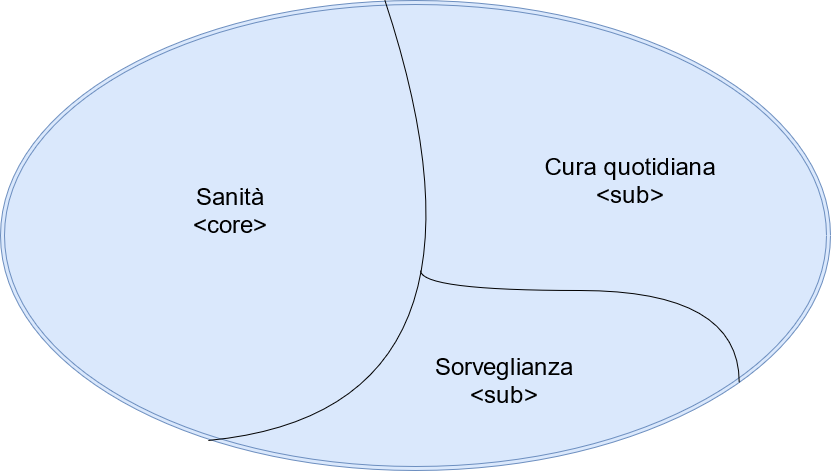
\includegraphics[width=0.5\textwidth]{DrawIo/domainsMap.png}
    \end{figure}
    
    Sono stati identificati tre domain, dove:
    \begin{itemize}
        \item \textbf{Sanità} è il \textbf{core domain}. Contiene tutta la logica e le funzioni utili a determinare lo stato di salute dell'animale, partendo dai soli dati vitali.
        
        \item \textbf{Cura quotidiana} è il \textbf{support domain}. Tramite la cura e le informazioni ricavate dalle azioni quotidiane dell'animale supporta il \textbf{core domain} nell'analisi di anomalie quali patologie, problemi di salute o comportamentali.
        
        \item \textbf{Sorveglianza} è il sub domain relativo alla gestione e monitoraggio video del canile.
    \end{itemize}
    
    \section{Identificazione dei Subdomain}
    Una volta individuato il core-domain, sono emersi anche i domini secondari e i sottodomini. 
    Sono stati definiti i seguenti subdomain:
    \begin{itemize}
        \item \textbf{Cura quotidiana:} racchiude tutti gli aspetti che riguardano la quotidiana gestione dei cani. Rientrano in questo sotto-dominio il \textbf{nutrimento} e ciò che è strettamente collegato ad esso, ovvero la \textbf{distribuzione} del cibo, il \textbf{consumo} e la rilevazione di \textbf{anomalie} nell'alimentazione.  
        \item \textbf{Sanità:} rappresenta tutto ciò che è collegato al \textbf{monitoraggio} della salute del cane e alla rilevazione di \textbf{anomalie} che necessitano di attenzione medica.
        \item \textbf{Sorveglianza:} riguarda il monitoraggio del canile mediante \textbf{videocamera} che è utile non solo per aspetti legati alla \textbf{sicurezza} ma anche per la stretta \textbf{sorveglianza} delle condizioni dei cani prossimi al parto o che hanno una situazione sanitaria che richiede una vigilanza continua anche nelle ore notturne.
    \end{itemize}
    Particolare attenzione è stata fatta a creare i sottodomini per il replacement piuttosto per il riuso.
    
    %TABELLA SUBDOMAIN
    \begin{figure}[H]
        \caption{Subdomains}
        \centering
        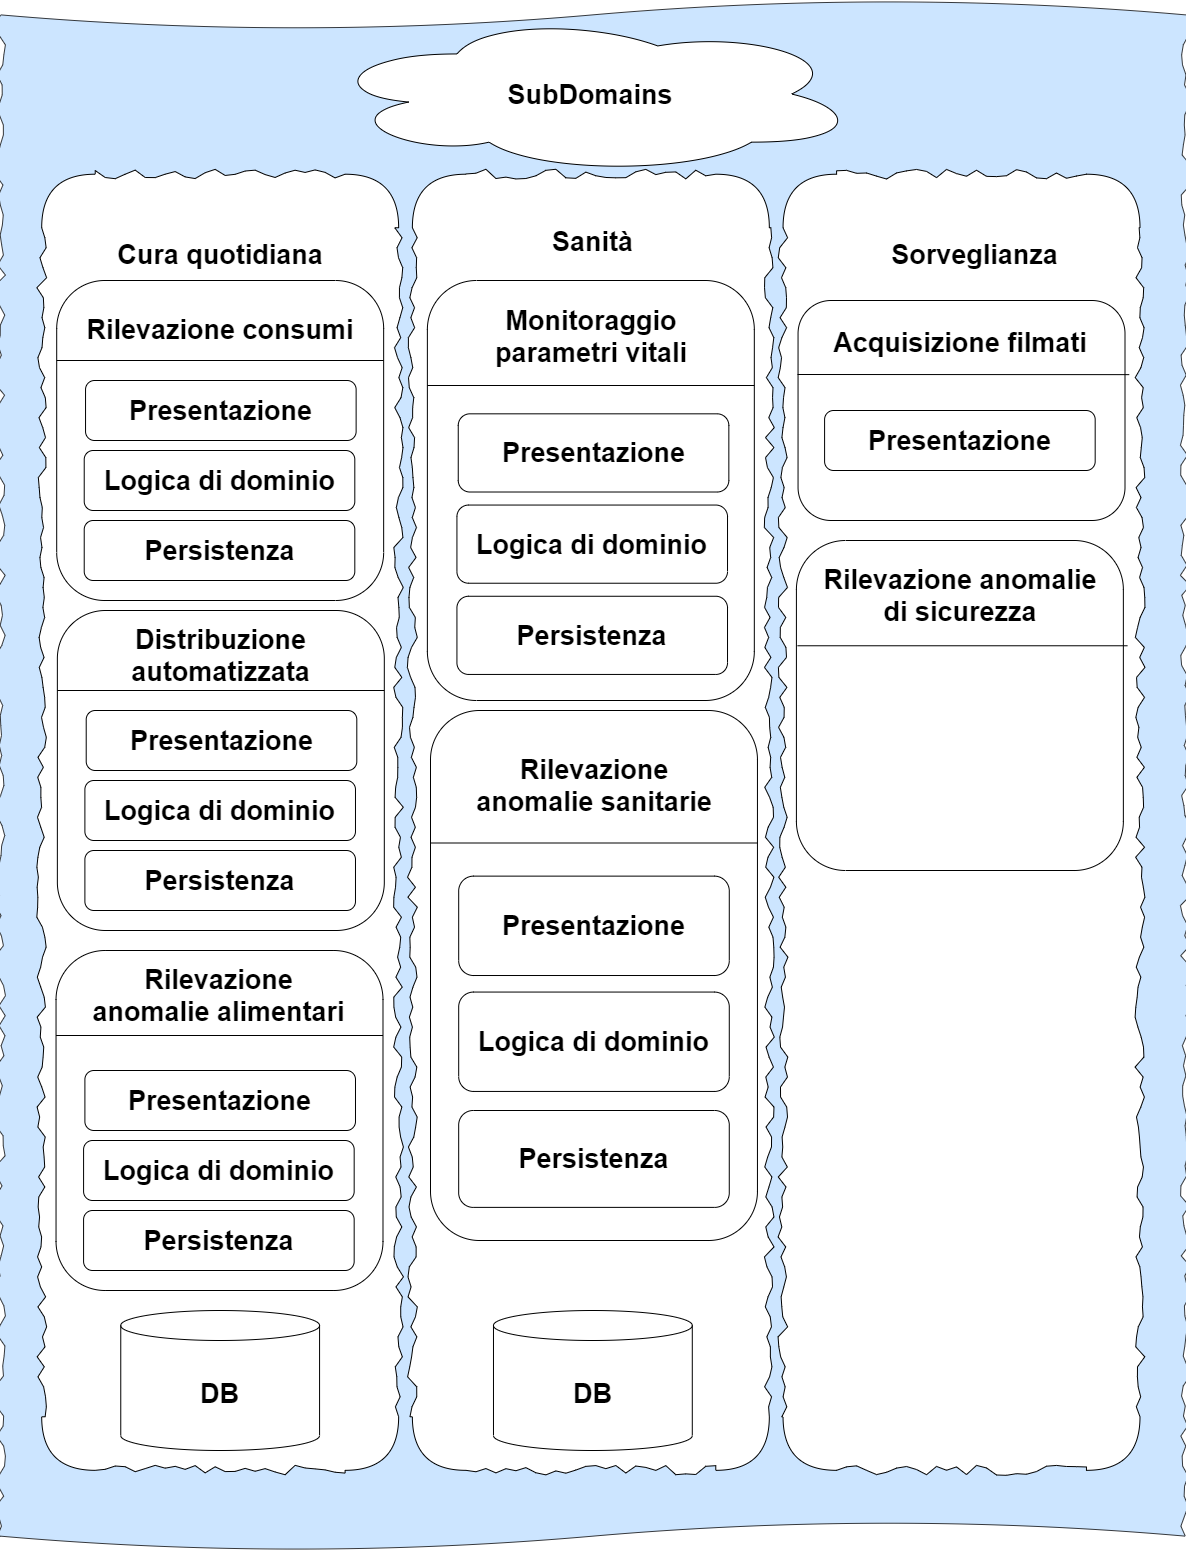
\includegraphics[width=0.8\textwidth]{DrawIo/subDomainsView.png}
    \end{figure}
    
    \section{Definizione dei Bounded Context}
    Un altro importante step è il riconoscimento dei Bounded Contexts. In questa fase il focus è incentrato sul confine tra i moduli individuati in precedenza. Lo scopo è di trovare delle porzioni isolate con confini ben definiti. L’isolamento deve essere non di funzionalità tecnica ma di dominio. Questo paradigma è riconoscibile anche nel trend attuale dei micro-servizi, che, tuttavia sono costruiti attorno ai confini di deployment, non del modello. Ciò assicura l’integrità e la facile scalabilità.
    Il modello del dominio infatti cresce in complessità nel tempo. Questo accade soprattutto nella filosofia Agile che abbraccia il cambiamento. Una continua revisione e raffinamento vengono portati avanti durante tutto l'arco della durata del progetto, per soddisfare differenti business use cases e nuove richieste del cliente. 
    Multipli team che lavorano allo stesso modello, inoltre, possono intralciarsi a vicenda e creare incomprensioni divergenti, a causa delle ambiguità nel linguaggio. 
    Queste sono le sfide avendo un single model, ed è per questo che è meglio avere più contexts/subdomains.
    Nello schema sottostante i Bounded Contexts sono stati collocati, assieme ai SubDomains che li contengono, in base alla loro complessità e alla relativa Business Differentiation. 
    
    %TABELLA BOUNDED CONTEXTS
    \begin{figure}[ht]
        \caption{Bounded Contexts}
        \centering
        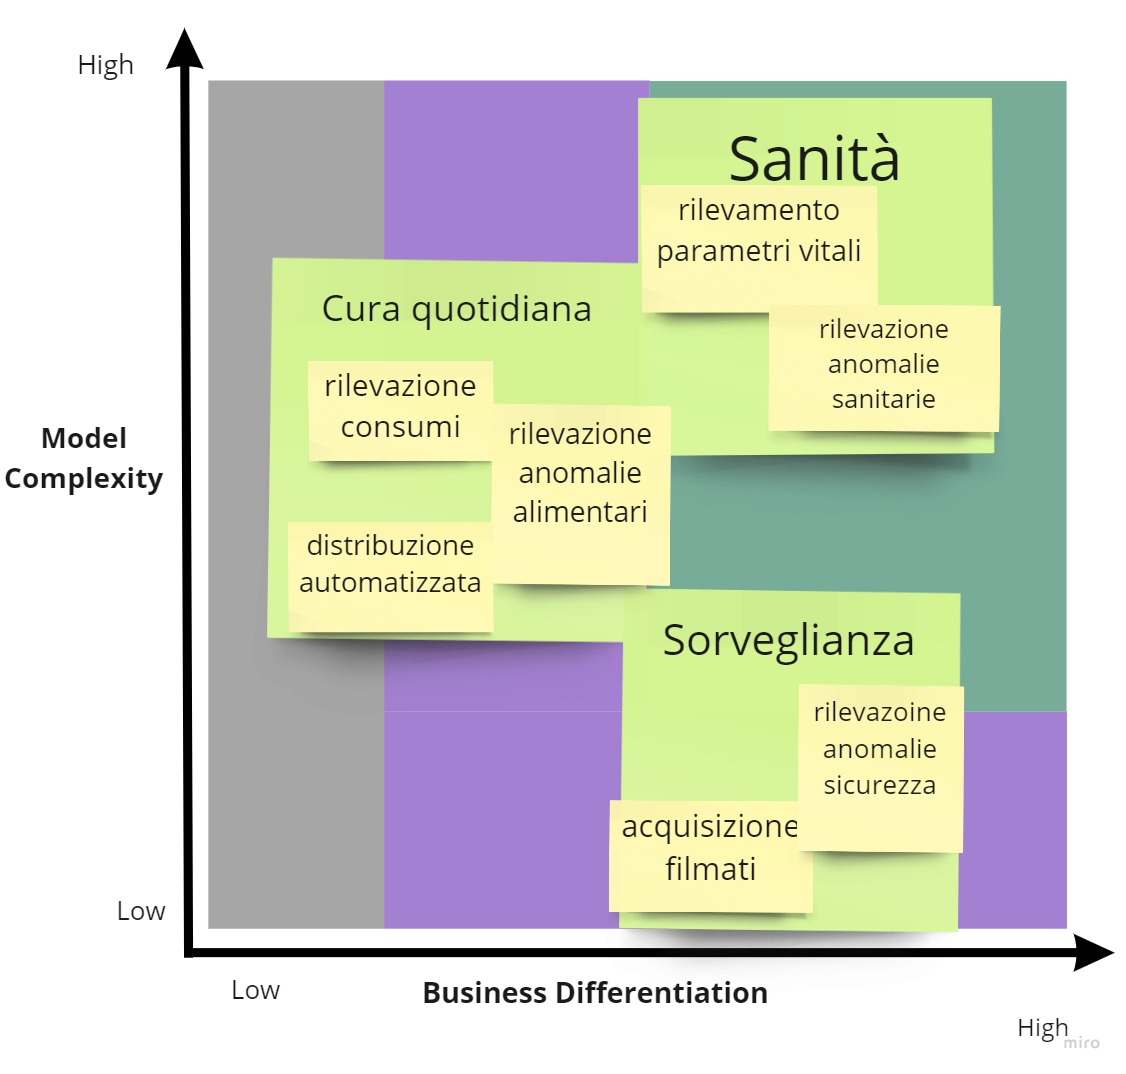
\includegraphics[width=0.8\textwidth]{Miro/BoundedContext.jpg}
    \end{figure}
    
    \section{Definizione delle Context Map}
    Avendo individuato nel sistema ci sono più Bounded Context, è importante riconoscere come dialogano. Creare una mappa concettuale [Fig. \ref{fig:ContextMap}] per definire i rapporti tra i Bounded Contexts è essenziale per il mantenimento del codice e dei vincoli di isolamento. La mappa, durante lo sviluppo, rappresenta lo stato presente e evolve in sincrono con il sistema stesso, più che rappresentare lo stato ideale futuro. Questo permette di chiarire anche agli eventuali team responsabili dei Bounded Context, i punti di contatto.
    
    Il livello scelto è molto più vicino al business, al Domain Problem, che al software. Nonostante ciò non è stata tralasciata la visione della parte implementativa, che comunque dovrà rispecchiare questo modello. Si può notare ciò dalla doppia suddivisione dello schema, sia dal punto di vista dei Sub-Domains, indicati in giallo, che dal punto di vista delle macro-componenti del sistema, indicate a sinistra. 
    
    Nella parte fisica, in tutti e tre i sub-domains, troviamo dei contesti che fungono da "supplier" verso altri. Le relazioni tra Bounded Contexts infatti sono state definite seguendo il più possibile i pattern del DDD. In questo caso si nota una Upstream/Downstream Relationship: è stato definito chi è il context customer o chi supplier in base al contesto che fornisce il flusso di informazioni e quello che le riceve. 
    La distribuzione automatizzata è composta da due sottocontesti, uno relativo al cibo erogato e misurato e l'altro all'acqua.
    Nei primi due casi i dati, essendo i dati trasmessi di grandezza esigua e di facile memorizzazione, vengono trasmessi ai contesti che si occupano della rilevazione e archiviazione degli stessi. Questi due Bounded Context condividono necessariamente uno Shared Kernel, i dati rilevati appartengono infatti allo stesso concetto del modello, ossia all'animale. 
    Essendo la distribuzione del cibo personalizzata in base alla classe dell'animale, un ulteriore contesto relativo alla gestione dei consumi è stato necessario, poichè attivamente definisce quali quantità erogare all'animale.
    Il flusso video, d'altra parte, data la mole di dati ha come customer direttamente la rilevazione delle anomalie della sicurezza. Questo Bounded Context, assieme agli affini che rilevano anomalie sanitarie e nei consumi, dopo aver preso in ingresso i dati, avvisano delle irregolarità il sistema delle notifiche. Questo passaggio è stato effettuato per mezzo di un "Open Host - Service" che espone le funzionalità del sistema notifiche.

    \subsection{Bounded Context Integration}
    Come specificato, è emersa la necessità di integrare dal punto di vista logico i due Bouned Context relativi ai consumi, nonostante si sia cercato di mantenerli il più possibile autonomi. L'integrazione infatti non deve avvenire mai prima a livello di codice, ma deve dipendere da un'integrazione a livello concettuale. 

    %TABELLA CONTEXT MAP
    \begin{figure}[ht]
        \caption{Context Map}
        \label{fig:ContextMap}
        \centering
        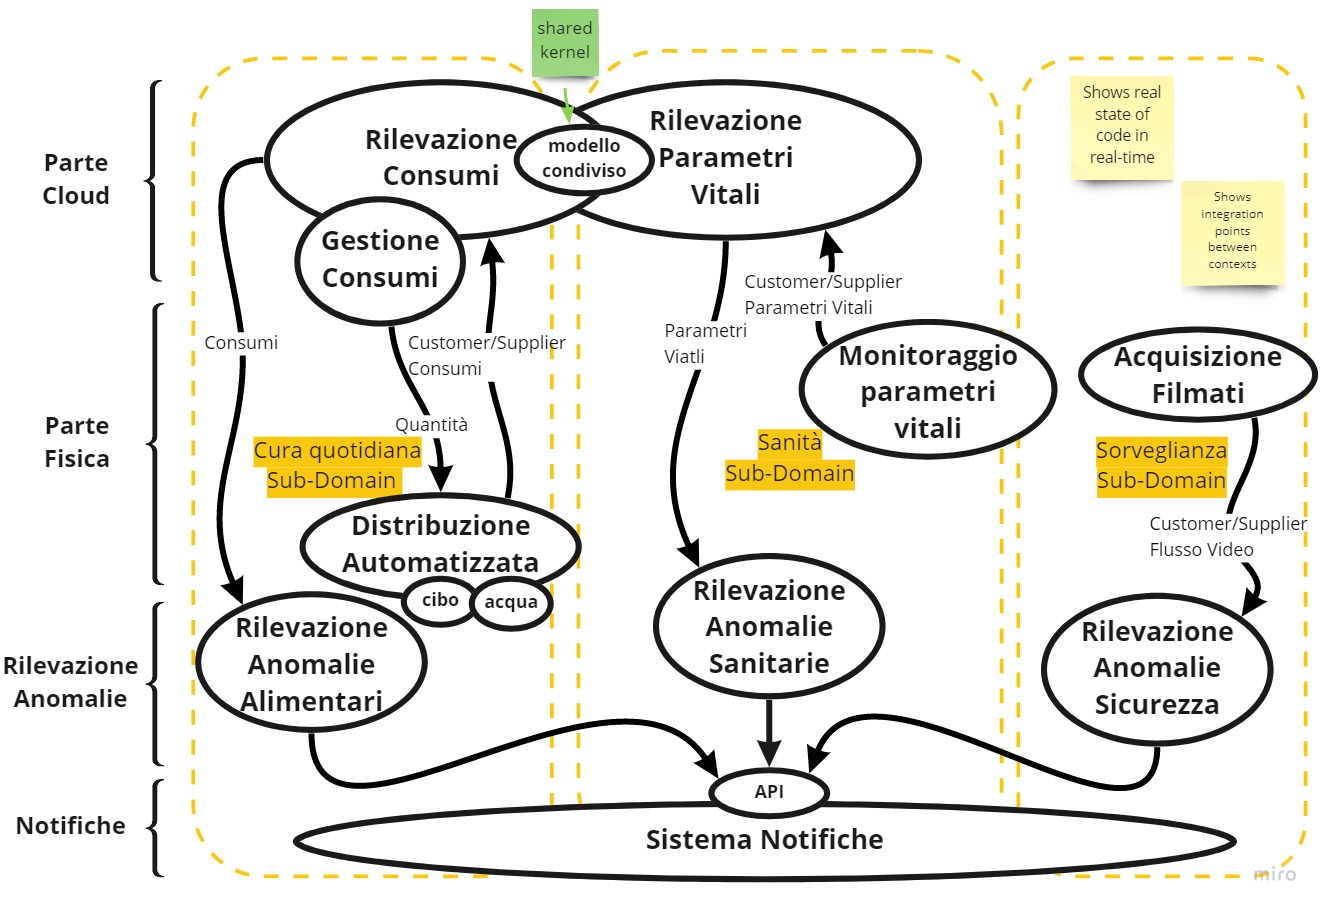
\includegraphics[width=0.9\textwidth]{Miro/ContextMap.jpg}
    \end{figure}
    